\documentclass[10pt,letterpaper]{article}
\usepackage[margin=0.7in]{geometry}
\usepackage[T1]{fontenc}
\usepackage{lmodern,graphicx,booktabs,longtable,array,amsmath,url,hyperref,caption}
\def\UrlBreaks{\do\/\do-\do\_\do.}
\hypersetup{colorlinks=true,urlcolor=blue,linkcolor=blue,pdftitle={Independent double-difference tomography: progress assessment}}
\setlength{\parindent}{0pt}
\setlength{\parskip}{5pt}
\setlength{\emergencystretch}{2em}
\captionsetup{font=small,labelfont=bf}
\newcommand{\repo}{https://github.com/nts345045/zhang-thurber-2003-independent-reproduction}
\begin{document}
\begin{center}
{\Large Independent double-difference tomography:\\progress and spending assessment}\par
13 October 2026\quad$\vert$\quad Zhang and Thurber (2003)\par
\small Assessed revision \texttt{684cb6a9f3ba}; main assessment pp.\ 1--4.
\end{center}

\textbf{Decision: stop open-ended model development.}
The independent implementation recovers coupled velocity and source perturbations in a homogeneous control, and preserves useful identified earthquake observations. It has not established the manuscript's Hayward fault geometry or velocity contrast. The immediate obstacle is failure of heterogeneous ray calculations during inversion. Four recent attempts have now stopped after 44--63 hours each. Further waiting or repeating them is not a scientific remedy. At most, approve the bounded human-led review on page 4 before funding another calculation.

\textbf{What works.}
The C++/OpenMP calculation predicts arrivals as origin time plus the path integral of slowness. Absolute and differential times constrain sources and gridded P-wave velocity together through ray bending and regularized least squares. Recomputed saved results for a 16-source, 6~km/s homogeneous control give:

\begin{center}\begin{tabular}{lrr}\toprule
Quantity & Initial & Recovered\\\midrule
Median 3D location error (km) & 0.1821 & 0.0210\\
Median velocity error, 203 illuminated nodes (km/s) & 0.3000 & 0.00795\\
Absolute arrival RMS (s; saved residual summary) & 0.3521 & 0.00635\\\bottomrule
\end{tabular}\end{center}

These results support limited joint-inversion capability. They do not establish heterogeneous recovery or accurate field locations. Manuscript Figure 1's prescribed 4--6~km/s input profile also matches its saved samples exactly; that achievement is an input reconstruction. The existing inventory remains \textbf{one reproduced entry and 61 partial entries}.

\textbf{Relation to the manuscript.}
The published result is improved velocity and locations relative to standard tomography, together with concentrated Hayward seismicity and sharper velocity contrasts [P1]. The historical independent synthetic experiment partly recovers the relative ranking: interior mean absolute velocity error is 0.313~km/s for standard tomography and 0.214~km/s for DD, compared with published values 0.245 and 0.178~km/s [P2]. Geometry, initial model and averaging mask differ, so these are reference scales, not matched agreement. Field concentration and sharpening remain unverified. No result here falsifies the published method.

\textbf{Useful retained capability.}
The authoritative selection contains 1,092 events, 37 physical stations, 14,262 P picks and 44,718 catalog differences, with event/pick resource IDs and channel SEED/FDSN identities. There are 98 normalized waveform differences. Identification and reproducible selection are valuable even if model development stops.

\newpage
\section*{Two generated figures: progress and its limits}
\begin{center}
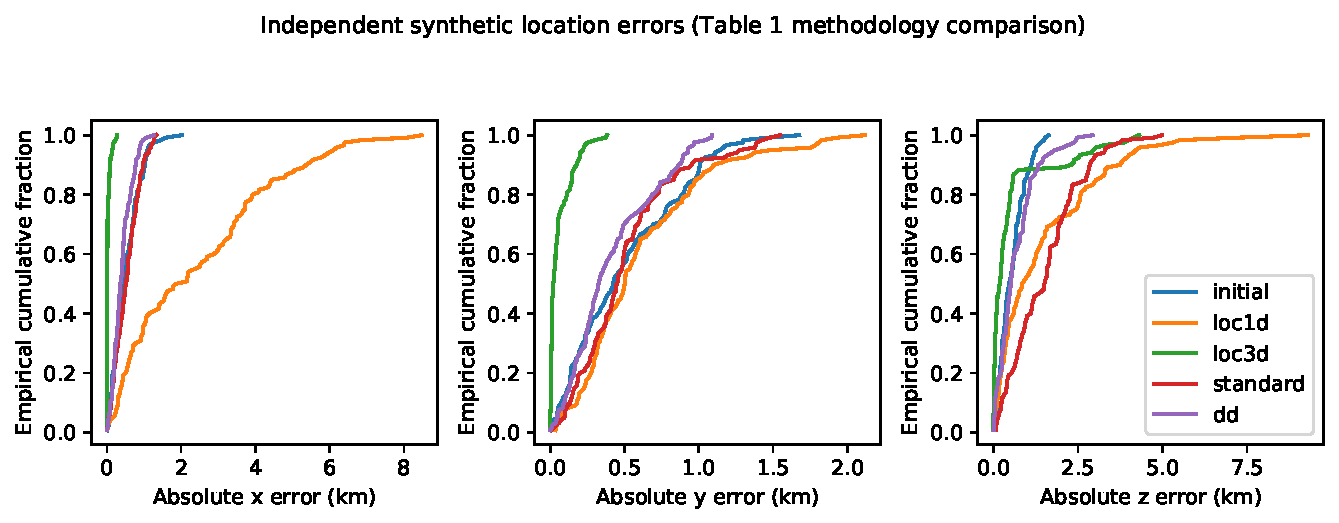
\includegraphics[width=0.98\linewidth]{figures/location_errors.pdf}
\captionof{figure}{Historical synthetic experiment, reused without regeneration. Curves show coordinate-error distributions for 120 invented test sources. DD (purple) improves on standard tomography (red), but 3D RMS error is 1.126~km, versus 1.112~km initially and 2.033~km for standard tomography. Fixed incorrect and known velocity models illustrate source--velocity coupling. These are not observations or a matched reproduction of Table 1.}
\end{center}
\vspace{3mm}
\begin{center}
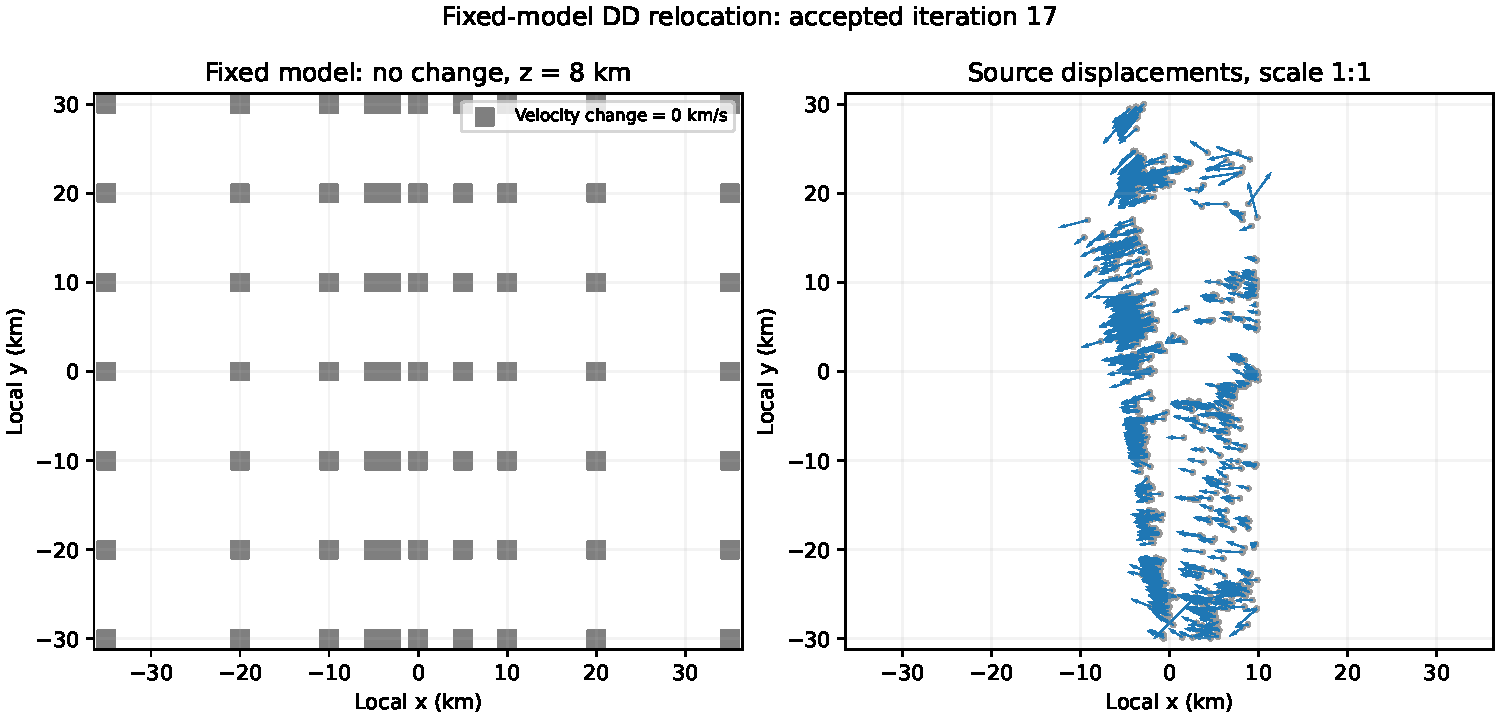
\includegraphics[width=0.98\linewidth]{data/development/hayward_comparison_saved_outputs_001/loc1d_001/comparison_figure.pdf}
\captionof{figure}{Completed fixed-model relocation of 1,092 authoritative events, accepted iteration 17. Velocity remains unchanged; horizontal displacement arrows use a 1:1 kilometre scale. Median and maximum 3D movements are 2.849 and 8.397~km. These are displacements from catalog locations, not errors against known truth. Completion of 18 updates does not establish nonlinear convergence. Full identifiers accompany the saved figure and tables [D2].}
\end{center}

\newpage
\section*{What now prevents a scientific conclusion}
\textbf{1. Forward-calculation reliability.}
All four formerly running inversions ended with the same failure: no objective could be evaluated after local ray rejection. Each final iteration rejected all 12 tested step fractions, down to $1/2048$. Saved histories and terminal trial records agree:

\begin{center}\begin{tabular}{lrr}\toprule
Attempt & Recorded updates / planned & Native wall time (h)\\\midrule
Standard, catalog only & 7 / 18 & 44.2\\
Clean catalog + waveform rebuild & 8 / 18 & 47.2\\
Catalog + waveform comparison & 8 / 18 & 54.1\\
Catalog DD & 9 / 18 & 63.2\\\bottomrule
\end{tabular}\end{center}

These overlapping jobs are failed calculations, not unfinished long-duration physical simulations. The combined and clean histories are identical, but their final geometries were not newly validated. The failure establishes an inability to evaluate updates under the implemented criteria; it does not isolate whether path representation, optimization or stopping criteria dominate.

\textbf{2. Experimental mismatch.}
The paper used 1,489 events, 52 stations, 20,257 absolute picks, 767,127 catalog differences and 17,955 waveform differences. The present waveform subset is only 0.55\% of that count. Exact cohort membership, historical elevations and the starting profile remain imperfectly matched. Assumed projections, receiver-depth conventions and numerical settings are disclosed departures, not calibrated equivalents. Instrument calibration responses are not required for normalized correlation.

\textbf{3. Incomplete recovery evidence.}
The original synthetic figures use procedural geometry, although manuscript Figure 2 was later replaced by authoritative geometry. A separate historical rebuild reports location RMS errors of 3.061~km (standard) and 1.388~km (DD), again exceeding the initial 1.112~km. Its saved metrics were inspected; its full raw result bundle was not rechecked here. A functioning program and lower weighted residuals therefore remain insufficient evidence of accurate reconstruction.

\textbf{Why the many checks have not settled this.}
Saved records pass 32 baseline and 48 later component checks, including homogeneous travel times, derivatives, cancellation and linear algebra. They do not establish heterogeneous mesh or nonlinear convergence. Initial-model full-DD covariance and individual-ray stationarity studies are additional capabilities; neither supplies a validated final inversion. Published Figure 11 used absolute arrivals at the DD model [P2], so a new full-DD covariance program is not a prerequisite for its counterpart.

\newpage
\section*{Spending decision and verification limits}
\textbf{Recommend no further autonomous model development now.}
The expected return from repeating multi-day inversions is low until a scientist selects a defensible, bounded forward-calculation test. Past expenditure is not evidence that another run will resolve this obstacle. Cohort ambiguity requires scientific judgment or missing information; additional computation cannot determine it.

\begin{center}\small
\begin{tabular}{@{}p{0.21\linewidth}p{0.75\linewidth}@{}}\toprule
\multicolumn{2}{l}{One optional next step, proposed for approval only}\\\midrule
Question & Can existing failures motivate one finite corrective experiment with scientific value?\\[4pt]
Work and deliverable & A tomography specialist reviews saved rejected trials and limiting-case evidence; produce a one-page stop/go decision and, only if justified, one specified benchmark. No implementation or simulation.\\[4pt]
Success criterion & Identify one failure class supported by saved records, one falsifiable corrective hypothesis and explicit truth-error/forward-accuracy thresholds before any new run is proposed.\\[4pt]
Principal risk & Another local diagnostic may not improve whole-data inversion; unpublished experiment choices may remain irreducible.\\[4pt]
Agent allowance & 0--10,000 additional tokens; hard ceiling 10,000. This is a planning allowance for file inspection and a short note, not a measured cost forecast. No new agents.\\[4pt]
Human and computing needs & At most two specialist hours; at most ten CPU-minutes of existing-file inspection, zero new simulations. These are scope ceilings, not inversion-time estimates.\\\bottomrule
\end{tabular}\end{center}

\textbf{Stopping condition.}
Stop at either ceiling or if no actionable hypothesis emerges. Archive the effort as a partial independent implementation unless a human explicitly approves a separate experiment. No dollar estimate is defensible without reconciled usage and applicable billing rates. The local goal counter reports 59.1 million tokens, but this is not an audited invoice or a reliable allocation of cost among experiments.

\textbf{Checks completed for this assessment.}
Saved-file arithmetic, identity checks and recorded-error comparisons support this assessment; Appendix B specifies their scope. Figures are existing outputs. No simulation, new agent or parameter search was launched.

\textbf{Checks left undone.}
No new mesh-convergence test, all-ray accuracy test, complete provenance audit or regeneration was performed. Panel references were checked, but not every image pair was visually re-compared. Earlier deliverables remain preserved; their ``running'' statements are superseded by these closed outcomes.

\clearpage
\appendix
\section{Panel inventory and evidence trail}

The existing convention gives 62 entries: 27 through Figure 9, 21 sections in Figure 10 and 14 in Figure 11. R denotes reproduced input-profile agreement; P denotes partial reproduction. I means independently imposed input, O means independently assembled authoritative observations, and M means independently calculated model output. Generation and agreement are separate classifications. No schematic is counted as a numerical result.

Figure 3 letters each cover the five generated depths (0, 3, 7, 11 and 16 km); correspondence to every inner published subplot was not established. Each grouped Figure 10/11 row enumerates all seven sections, $y=-30,-20,-10,0,10,20,30$ km, with identical status, evidence files and limitation. The CSV retains all 62 individual entries.

\small\setlength{\tabcolsep}{4pt}

\begin{longtable}{@{}p{0.115\linewidth}p{0.245\linewidth}p{0.06\linewidth}p{0.445\linewidth}p{0.055\linewidth}@{}}\toprule Panel & Quantity & Gen./\newline agree. & Quantitative comparison; limitation & Files\\\midrule\endhead

1 & Horizontal true P-velocity slice & I/R & Saved 4--6 km/s profile agrees with the coded written profile at every sample (maximum error 0 km/s). Input reconstruction, not inversion recovery; plotted extent/depth are independent choices. & E1\\[3pt]

2 & Synthetic-test event/station geometry and inversion grid & O/P & 724 catalog sources; 52 receiver epochs. No exact-cohort comparison. Original cohort and projection unmatched; geometry only. & E2\\[3pt]

3a & Standard tomographic P velocity & M/P & Baseline interior mean |velocity error| 0.313 km/s; paper 0.245 km/s uses an unmatched mask. L1 & E3a\\[3pt]

3b & DD tomographic P velocity & M/P & Baseline interior mean |velocity error| 0.214 km/s; paper 0.178 km/s uses an unmatched mask. L1 & E3b\\[3pt]

3c & True minus DD P velocity & M/P & Baseline interior mean |velocity error| 0.214 km/s; paper 0.178 km/s uses an unmatched mask. L1 & E3c\\[3pt]

3d & True minus standard P velocity & M/P & Baseline interior mean |velocity error| 0.313 km/s; paper 0.245 km/s uses an unmatched mask. L1 & E3d\\[3pt]

4 & network, catalog seismicity, and inversion grid & O/P & 1,092 events / 37 physical stations; paper 1,489 / 52. L2; input geometry only. & E3\\[3pt]

5a & event map: NCSN catalog & O/P & No matched error metric. L2 & E4\\[3pt]

5b & event map: standard tomography & M/P & No matched error metric. L2, L3 & E4\\[3pt]

5c & event map: DD location & M/P & No matched error metric. L2, L3 & E4\\[3pt]

5d & event map: DD tomography & M/P & No matched error metric. L2, L3 & E4\\[3pt]

6a & geographical map & O/P & No matched error metric. L2, L4 & E6\\[3pt]

6b & rotated Cartesian map & O/P & No matched error metric. L2, L4 & E6\\[3pt]

6c & across-strike depth section AA-prime & O/P & No matched error metric. L2, L4 & E6\\[3pt]

6d & along-strike depth section BB-prime & O/P & No matched error metric. L2, L4 & E6\\[3pt]

7a & standard: geographical map & M/P & No matched error metric. L2, L3, L4 & E7\\[3pt]

7b & standard: rotated Cartesian map & M/P & No matched error metric. L2, L3, L4 & E7\\[3pt]

7c & standard: across-strike depth section AA-prime & M/P & No matched error metric. L2, L3, L4 & E7\\[3pt]

7d & standard: along-strike depth section BB-prime & M/P & No matched error metric. L2, L3, L4 & E7\\[3pt]

8a & DD location: geographical map & M/P & No matched error metric. L2, L3, L4 & E8\\[3pt]

8b & DD location: rotated Cartesian map & M/P & No matched error metric. L2, L3, L4 & E8\\[3pt]

8c & DD location: across-strike depth section AA-prime & M/P & No matched error metric. L2, L3, L4 & E8\\[3pt]

8d & DD location: along-strike depth section BB-prime & M/P & No matched error metric. L2, L3, L4 & E8\\[3pt]

9a & DD: geographical map & M/P & No matched error metric. L2, L3, L4 & E9\\[3pt]

9b & DD: rotated Cartesian map & M/P & No matched error metric. L2, L3, L4 & E9\\[3pt]

9c & DD: across-strike depth section AA-prime & M/P & No matched error metric. L2, L3, L4 & E9\\[3pt]

9d & DD: along-strike depth section BB-prime & M/P & No matched error metric. L2, L3, L4 & E9\\[3pt]

10a (7 sections) & across-strike DD velocity & M/P & No matched error metric. L2, L3; no quantitative validation of sharpening. & E10\\[3pt]

10b (7 sections) & across-strike standard velocity & M/P & No matched error metric. L2, L3; no quantitative validation of sharpening. & E10\\[3pt]

10c (7 sections) & across-strike DD minus standard velocity & M/P & No matched error metric. L2, L3; no quantitative validation of sharpening. & E10\\[3pt]

11a (7 sections) & resolution-matrix diagonal & M/P & No matched error metric. L2, L5 & E11\\[3pt]

11b (7 sections) & interpolated nodal conditional velocity noise from independent picks & M/P & No matched error metric. L2, L5 & E11\\[3pt]

\bottomrule\end{longtable}\normalsize

\subsection*{Limitation keys}

\noindent\textbf{L1.} Historical synthetic geometry and homogeneous starting model differ from the paper; sampling masks are unmatched and production ray convergence fails. Figure 2 was later replaced with authoritative geometry, but Figure 3 was not rerun on it.\par\smallskip

\noindent\textbf{L2.} Authoritative independent subset, not the original cohort: 1,092 versus 1,489 events and 37 versus 52 stations. Uncertain study membership, historical receiver elevations, selection, projection and starting profile remain disclosed assumptions.\par\smallskip

\noindent\textbf{L3.} Legacy calculated field solution, not a validated Earth model. Forward-calculation errors and unresolved nonlinear convergence limit interpretation; no independent true hypocenters or quantitative published-image comparison.\par\smallskip

\noindent\textbf{L4.} Published section-box and fault-trace geometry were not recovered from written specifications. Both depth views use all selected zoom events; sections are not exact manuscript selections.\par\smallskip

\noindent\textbf{L5.} Absolute-pick resolution at the legacy DD estimate uses independent regularization and covariance assumptions. It excludes ray/model errors and active bounds. Interpolated nodal noise is not uncertainty of an interpolated velocity. It is not a validated final corrected model.\par\smallskip

\subsection*{Supplementary scope}

No supplementary panel was identified in the original SSA issue contents or abstract listing, rechecked on 13 October 2026. Thus there is no documented supplementary panel identifier to inventory; this does not establish that no ancillary material exists elsewhere. Supplementary reproduction remains unspecified, rather than silently counted as successful.

\subsection*{File references}

Paths are relative to the repository root. Files were checked for existence. E2 preserves the generated geometry through its manifest and validation record; its data members are listed there. The individual numerical and provenance checks actually performed are specified in \path{data/progress_assessment_2026-10-13/evidence.json}. Uninspected content is not certified by existence alone.

\footnotesize

\noindent\textbf{E1} Data: \path{data/synthetic/truth_slice.csv}.\par Plot: \path{figures/figure01.pdf}.\par\medskip

\noindent\textbf{E2} Data: \path{data/development/loma_geometry_figure_001/inputs/truth_events.csv}, \path{data/development/loma_geometry_figure_001/inputs/stations.csv}, \path{data/development/loma_geometry_figure_001/inputs/initial_grid.csv}, \path{data/development/loma_geometry_figure_001/manifest.json}.\par Plot: \path{data/development/loma_geometry_figure_001/figure02_authoritative_geometry_candidate.pdf}.\par\medskip

\noindent\textbf{E3} Data: \path{data/hayward/initial_events.csv}, \path{data/hayward/stations.csv}, \path{data/hayward/selection_manifest.json}.\par Plot: \path{figures/hayward/figure04_geometry.pdf}.\par\medskip

\noindent\textbf{E4} Data: \path{data/hayward/initial_events.csv}, \path{data/hayward/standard_events.csv}, \path{data/hayward/loc1d_events.csv}, \path{data/hayward/dd_events.csv}, \path{data/hayward/figure_metrics.json}.\par Plot: \path{figures/hayward/figure05_locations.pdf}.\par\medskip

\noindent\textbf{E10} Data: \path{data/hayward/vertical_sections.csv}, \path{data/hayward/standard_grid.csv}, \path{data/hayward/dd_grid.csv}, \path{data/hayward/figure10_velocity_manifest.json}.\par Plot: \path{figures/hayward/figure10_velocity.pdf}.\par\medskip

\noindent\textbf{E11} Data: \path{data/hayward/resolution_sections.csv}, \path{data/hayward/absolute_resolution.csv}, \path{data/hayward/absolute_resolution_manifest.json}.\par Plot: \path{figures/hayward/figure11_resolution.pdf}.\par\medskip

\noindent\textbf{E3a} Data: \path{data/synthetic/standard_slices.csv}, \path{data/synthetic/standard_events.csv}, \path{data/metrics.json}.\par Plot: \path{figures/figure03a.pdf}.\par\medskip

\noindent\textbf{E3b} Data: \path{data/synthetic/dd_slices.csv}, \path{data/synthetic/dd_events.csv}, \path{data/metrics.json}.\par Plot: \path{figures/figure03b.pdf}.\par\medskip

\noindent\textbf{E3c} Data: \path{data/synthetic/dd_slices.csv}, \path{data/synthetic/dd_events.csv}, \path{data/metrics.json}.\par Plot: \path{figures/figure03c.pdf}.\par\medskip

\noindent\textbf{E3d} Data: \path{data/synthetic/standard_slices.csv}, \path{data/synthetic/standard_events.csv}, \path{data/metrics.json}.\par Plot: \path{figures/figure03d.pdf}.\par\medskip

\noindent\textbf{E6} Data: \path{data/hayward/initial_zoom_events.csv}, \path{data/hayward/initial_geographic_events.csv}.\par Plot: \path{figures/hayward/figure06_initial.pdf}.\par\medskip

\noindent\textbf{E7} Data: \path{data/hayward/standard_zoom_events.csv}, \path{data/hayward/standard_geographic_events.csv}.\par Plot: \path{figures/hayward/figure07_standard.pdf}.\par\medskip

\noindent\textbf{E8} Data: \path{data/hayward/loc1d_zoom_events.csv}, \path{data/hayward/loc1d_geographic_events.csv}.\par Plot: \path{figures/hayward/figure08_loc1d.pdf}.\par\medskip

\noindent\textbf{E9} Data: \path{data/hayward/dd_zoom_events.csv}, \path{data/hayward/dd_geographic_events.csv}.\par Plot: \path{figures/hayward/figure09_dd.pdf}.\par\medskip

\normalsize

\section{Supporting checks, provenance and references}
\textbf{Repository and state.}
\href{\repo}{Zhang--Thurber independent reproduction}, assessed main revision:\par
\texttt{684cb6a9f3bad6c7d6a63666c17ae566454ca3fe}.\par
The retained inversion worktree is revision:\par
\texttt{1d22e2b2de60315154343bdcec692769a174e3cb}.\par
At assessment start, tracked main files were clean; the user's
\path{pause_and_evaulate_prompt.md} was untracked. It is left unchanged and is not part of this publication.
Only this assessment and its supporting records are added. No previous figure,
report, solver, configuration or dataset is replaced.

\textbf{D1: quantitative checks.}
Recomputed synthetic source errors and velocity-error means; checked the
prescribed profile; verified 19 fixed-model package hashes and its 18-row
history; recomputed field displacements; checked identity fields across
58,980 catalog rows; counted 98 waveform differences; and joined failed-run
histories to their hashed trial records. No new physical calculations were made.
\path{data/progress_assessment_2026-10-13/evidence.json} records calculated
statistics, original file hashes, check scope and explicit omissions.
The eight CSV files beside it preserve the four failed histories and their final
trial tables. Histories are byte-preserved; trial \path{failure_prefix} values
are reduced to basenames to omit local machine paths. Numerical cells remain
unchanged. Original file hashes and sanitized closure summaries retain the
evidence trail; private process receipts remain local.
Two owned execution sessions returned code 1. The other two stored controllers
record launcher reaping and bind the inner failed records, with no live group
members; all four native processes were absent. The original DD bootstrap's
external terminal status remains unknown because its receipt is stale.
That limitation is not relabeled as successful external reaping.

\textbf{D2: field figure and identities.}
\path{data/development/hayward_comparison_saved_outputs_001/loc1d_001/}
contains \path{event_points.csv}, \path{model_nodes.csv},
\path{receiver_epochs.csv}, the figure and identifier sidecars,
\path{source_tables.tar.gz}, \path{source_path_mapping.json}, and the checked
\path{manifest.json}. The displayed events retain event/origin resource IDs;
channel metadata and differential observations retain their full mappings.
\path{progress_assessment.pdf.identifiers.json} links the reused figure to these
identified source tables. No historical response was backdated.

\textbf{D3: historical controls.}
\path{data/joint_recovery/} contains homogeneous truth, initial and recovered
event/grid tables and \path{dd_coverage.csv}.
\path{data/synthetic/} contains the 120-source baseline tables plotted here;
\path{data/metrics.json} and \path{data/validation.csv} summarize that baseline.
The distinct later results are in
\path{data/development/historical_clean_rebuild_001/results/data/metrics.json}
and \path{data/development/historical_clean_rebuild_001/results/data/validation.csv}.
Their numbers are not substituted into the older figures.

\textbf{D4: selection and additional diagnostics.}
\path{data/hayward/selection_manifest.json}, \path{data/hayward/observations.csv},
\path{data/hayward/stations.csv}, and \path{data/development/native_dt_cc_001/dt.cc}
support the input counts. The CC identifier roster and epoch tables accompany
that export. Initial full-DD uncertainty evidence is retained in
\path{data/development/hayward_initial_full_dd_resolution_001/}; it was not
recomputed here. Reference-path existence is not a full independent audit of
the large resolution matrices.

\textbf{Provenance assessment.}
Inspected figures arise from independent code, declared synthetic inputs, or
authoritative observations. No copied publication image or authors' numerical
output was found among the figures and inputs inspected here. This limited
inspection is not an exhaustive provenance certification. The principal
documented problem is unmatched experimental geometry and legacy results with
failed numerical checks, not an established instance of copied data. Written
publication values are comparison references; no plot digitization was used.
No schematics are included as reproduced results.

\textbf{P1.} Zhang, H., and C.~H. Thurber (2003), Double-Difference Tomography:
The Method and Its Application to the Hayward Fault, California,
\emph{BSSA} 93, 1875--1889,
\href{https://doi.org/10.1785/0120020190}{doi:10.1785/0120020190}.
\href{https://www.seismosoc.org/Publications/BSSA_html/bssa_93-5/02190.html}{Original SSA abstract}.

\textbf{P2.} \href{https://www.researchgate.net/publication/215754286_Double-Difference_Tomography_The_Method_and_Its_Application_to_the_Hayward_Fault_California}{Author-posted manuscript text}:
synthetic velocity errors and Table 1, pp.\ 1878--1879; absolute-arrival
resolution analysis, p.\ 1884. Only written specifications and numerical
reference statements were consulted, not authors' code or figure files.

\textbf{P3.} \href{https://www.seismosoc.org/Publications/BSSA_html/bssa_93-5/ssa_toc_93-5.html}{SSA October 2003 issue contents};
supplement listing checked with P1 on 13 October 2026.
See also \path{reference/specification_notes.md} for the earlier search scope.

\end{document}
